\section{Proposed Matheuristics}
\label{sec:method}

The proposed solution method for the thermal UCP 
consists of two phases: a construction phase, where
an initial feasible solution is built, and an
improvement phase, where five procedures,
including KS and four tailored-made versions of LB,
are applied to the constructed solution.
In the remainder of the section, all these
components are further explained.



\subsection{Construction Phase}
\label{construction}

To the best of our knowledge, the best construction
method for UCP is due to \citet{Harjunkoski2021}.
Their heuristic, referred as HGPS, is of the type relax and fit (R\&F).
The solution strategy of R\&F methods is to reduce the size of the MILP to a smaller, easier-to-solve model called subproblem, fixing those variables likely to keep their values in the optimal solution and letting the solver decide among the others. Finally, the subproblem is input into the solver, expecting that the solver returns a high-quality solution.
Our idea is to develop am enhanced R\&F heuristic that
better exploits the structure of our problem.


%I. Harjunkoski and M. Giuntoli and J. Poland and S. Schmitt
The HGPS heuristic
begins by solving a linear relaxation of the UCP, obtaining a solution $\tilde{x}$. In this method, the variables $u_{g,t}$ to be fixed to one in the subproblem are those that satisfy the condition $\tilde{u}_{g,t}\cdot\tilde{p}_{g,t} \geq \underline{P}$. We will call this condition: Harjunkoski's rule. Let $\tilde{u}_{g,t}$ and $\tilde{p}_{g,t}$ be the values taken by the variables in the linear relaxation solution. Once the variables are fixed, the subproblem is solved, deciding over the rest of the non-fixed variables. 

Our heuristic, named HARDUC,
starts by solving a linear relaxation of the UCP. Then, to form the subproblem, the variables $u_{g,t}$ that satisfy the criterion $\tilde{u}_{g,t}\cdot\tilde{p}_{g,t}=0$ are fixed to zero, and the decision over the other variables is left to the solver.
%\The value of the variables $u_{g,t}$ obtained from the linear relaxation of the problem is represented by $\tilde{u}_{g,t}$.


%\hl{Discuss this paragraph}
Figure \ref{fig:Constructives} illustrate the difference between these two heuristics, indicating the space of ${u}_{g,t}$ variables. On the left-hand side, we see the HGPS method, where the shaded region indicates variables set to one, and the light region shows variables yet to be determined by the solving the subproblem. On the right-hand side, we have the HARDUC method, where the light region comprises non-zero variables according to Harjunkoski's rule but with a value greater than $\underline{P}$. Finally, the variables that meet the criterion ${u}_{g,t}: \{ \tilde{u}_{g,t}\cdot \tilde{p}_{g,t} < \underline{P} \} \cap \{\tilde{u}_{g,t}\cdot\tilde{p}_{g,t}\neq 0\}$ will be used for the construction of a restricted candidate list (RCL). We expect these variables are more likely to be in the optimal solution than those with zero values. This RCL is essential for other improving methods based on local branching described in this work.

\begin{figure}[htb]
\centering
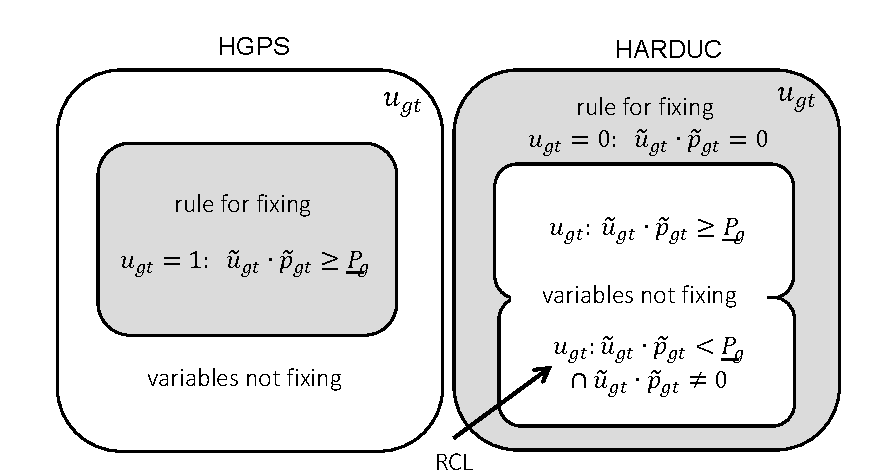
\includegraphics[width=14cm]{Figure/Contructives.pdf}
\scriptsize \caption{Rules for R\&F construction methods. The shaded area represents the subset of variables to be fixed in the subproblem.}
\label{fig:Constructives}
\end{figure}


After obtaining a feasible solution, the search for an improved solution starts as a second phase of the solution algorithm.  We develop a family of five metaheuristics, including one based on KS and four different versions of LB. All these methods are described in the following sections.

\subsection{Improvement Phase}
\label{metaheuristics}

Once an initial feasible solution has been obtained, an improvement phase is applied in order to improve the solution. For this purpose, two main solution frameworks are proposed and explained below.

\subsubsection*{Kernel Search}


Kernel search is a matheuristic initially developed by \citet{Angelelli2010} to solve a multidimensional knapsack problem with outstanding results. 
We have not seen any KS implementation for UCPs, to the best of our knowledge.
%RZ We envision KS as a highly competitive method for solving the UCP, so it was chosen as another matheuristics besides the four LB versions.
%
KS is divided into two phases: initialization and expansion. During the initialization phase, the binary variables in problem $P$ that are likely to take a value of one in the optimal solution are determined. This subset of variables is called the kernel (equivalent to the binary support in LB). The selection of the variables that form the kernel is usually those that take the value one in the linear relaxation.
%
Then, the remaining variables not part of the kernel are sorted according to some economic criterion (often, the reduced costs of the LP relaxation) and divided into small groups called buckets. 

The expansion phase consists of solving the multiple MILP subproblems formed by each bucket concatenated one by one with the kernel, one step at a time. This phase is called expansion because, in each iteration, bucket variables that take the value of one are picked and added to the kernel. The constraint  $\sum_{j\in B_{i}}x_{j} \geq 1$ must be added to the subproblem to enforce that at least one variable of the bucket takes the value one. Because of this constraint, the kernel tends to increase in size with each iteration. For each iteration, the remaining bucket variables that are not part of the subproblem must be fixed to zero. The conventional KS terminates when each bucket has been resolved with the kernel or the allowed time is met \citep{Angelelli2010}. % has timed out 

%\subsubsection*{Implementation of KS for the UCP}
\vspace{1em}\noindent\textit{Implementation of KS for the UCP}\\

We present a version of KS that can be seen in Algorithm \ref{alg:KS} called \texttt{kernelsearch()}. 
The inputs of algorithm \texttt{kernelsearch()} are total time ($\textit{t\_total}$),  a feasible solution ($\bar{x}$) of an instance of UCP to solve ($P$). The outputs are $x^{*}$ and $z^{*}$, respectively, the incumbent solution and its cost.
The function \texttt{kernelsearch()} starts the initialization phase by building the kernel from variables with $u_{g,t}=1$ in the feasible solution $\bar{x}$; this feasible solution is obtained from the constructive method HARDUC. 
It is noted that only the dominant variable $u_{g,t}$ is used for building both the kernel and the buckets. 
Note that our version of KS does not require kernel building. KS is only used as an improvement method, as a constructive method that determines the kernel.

\begin{algorithm}[htb]
\small
\caption{\texttt{kernelsearch()}}
\label{alg:KS}
\begin{algorithmic}
%\fontsize{10}{8}\selectfont 
\Require \\
$\bar{x}$=a feasible solution of $P$, \\
$P$=a formulation of the instance to solve,\\
$\textit{t\_total}$
\Ensure \\
A feasible solution $x^{*}$ of value $z^{*}$ \\

\While{$(elapsed\_time < t\_total)$}
    %\State \hfill
    \State $\textit{cutoff} \leftarrow z^{*}$ \Comment{\textbf{Initialization phase}}
    \State $K \leftarrow$ kernel formed from the variables that fulfill $u_{g,t}:u_{g,t}=1\in\bar{x}$ 
    \State $ P^{ K}\leftarrow$ \texttt{fixing}(1,$K$,$P$) fixing to 1 all the variables into kernel
    \State $\lbrace \hat{x}, \hat{z} \rbrace \leftarrow \texttt{solveLR}( P^{\text{fix(\textit{K})}})$ 
    \State $U \leftarrow$ select the variables that fulfill ${u}_{g,t}\notin K$
    \State $\textit{nbucks} \leftarrow 1 + 3.322 \ln(|\textit{U}|)$
    \State $U^{\text{ord}} \leftarrow$ sort $U$ in ascending order of reduced cost (most negative first) 
    \State $\{ B_i\}_{i=1}^{\textit{nbucks}} \leftarrow$ \texttt{buildbuckets}($U^{\text{ord}}$,$\textit{nbucks}$)  
    \State $tl \leftarrow (\textit{t\_total}-\textit{elapsed\_time}) / n$ 
%RZ    \State \hfill\Comment{\textbf{Expansion phase}}
    \For{($i=1,\textit{nbucks}$)} \Comment{\textbf{Expansion phase}}
            \State $ P^{ K\cup B_i}\leftarrow$ \textbf{fixing}(0,$\overline{B}_i$,$P$) \Comment{fixing to 0 all variables of the other buckets}
            \State $ P^{ K\cup B_i}\leftarrow$ $ P^{ K\cup B_i} \cup \lbrace \sum_{j\in B_{i}}x_{j} \geq 1\rbrace $ \Comment{A variable from the bucket is forced into entering the kernel}
            \State $\lbrace stat, \widetilde{x}, \widetilde{z} \rbrace \leftarrow \texttt{solve}( P^{ K\cup B_i}, \textit{cutoff},tl)$
            \If{(stat = \text{feasible})}
                    \If{$(\widetilde{z} < z^{*} )$} 
                        \State $z^{*} \leftarrow \widetilde{z}$ \Comment{Update best known objective}
                        \State $\textit{cutoff} \leftarrow \widetilde{z}$ \Comment{Tighten cutoff for next iteration}
                        \State $x^* \leftarrow \widetilde{x}$ \Comment{Update best solution}
%                 \State $  \textit{cutoff} \leftarrow z^{*} \leftarrow \widetilde{z}$; $x^* \leftarrow \widetilde{x}$ \hl{ALGO AQUI NO ENCAJA... triple arrow?? UILL - LO CAMBIÉ ARRIBA EN TRES LINEAS EN AZUL Y LO COMENTE PARA ACLARAR CADA LINEA}
                \EndIf
                \State $K \leftarrow$ update the kernel with the variables in $B_i$ such that $u_{g,t} = 1$ in $\widetilde{x}$.
%                \State K $\leftarrow$ update the kernel from the buckets variables that fulfill $\{u_{g,t}:u_{g,t}=1\in\bar{x}\}$ \hl{RZ esta expesion no es correcta UILL doc... la cambie por la de arriba }
            \EndIf
    \EndFor
\EndWhile\\
\Return{$x^{*}$}
\end{algorithmic}
\end{algorithm}          


The construction of the buckets begins by fixing to $1$ the variables constituting the kernel $u_{g,t} \in K$ and solving a linear relaxation of the problem $P^\text{fix(\textit{K})}$.
Then, the set $U$ is constructed with the variables $u_{g,t}$ that are not inside the kernel $K$.
The number of buckets is calculated using Sturges's rule \citep{Scott2009}: $\textit{nbucks}=1+3.322 \ln(|U|)$.

Then, the $u_{g,t}\in U$ variables are sorted in ascending order of their reduced costs obtained from the linear relaxation problem $P^\text{fix(\textit{K})}$, so the most negative reduced costs come first (since this is a minimization problem). The newly ordered set is denoted as $U^{\text{ord}}$.

The set of buckets of size $\textit{nbucks}$, into which the variables of set $U^{\text{ord}}$ are divided, is denoted as $B_i$, where $i$ is an index ranging from 1 to $\textit{nbucks}$.

%https://www.mdpi.com/2076-3417/12/22/11421
\begin{algorithm}[htb]
\small%\fontsize{10}{8}\selectfont 
\caption{\texttt{buildbuckets()}}
\label{alg:buildbuckets}
\begin{algorithmic}
\Require \\
$U^{\text{ord}}$=list of $u_{g,t}$ outside the kernel, most negative reduced cost first, \\
$\textit{nbucks}$=number of buckets
\Ensure \\A set of buckets $\{ B_i\}_{i=1}^{\textit{nbucks}}$\\
\State $\{ B_i\}   \leftarrow \lbrace\phi\rbrace$
\State $\textit{start}      \leftarrow 0 ; \textit{end}  \leftarrow 0$
\State $n                \leftarrow |U^{\text{ord}}|$
\State $k                \leftarrow \lfloor n / \textit{nbucks}\rfloor$
\State $\textit{remainder} \leftarrow n \mod{(\textit{nbucks})}$ 
    \For{ $i=1,\textit{nbucks}$} 
        \State $\textit{end} \leftarrow \textit{start} + k$
        \If{$\textit{remainder} > 0$} 
            \State $ \textit{end}       \leftarrow \textit{end} + 1$
            \State $ \textit{remainder} \leftarrow \textit{remainder} - 1$
        \EndIf            
        \State $ B_i\leftarrow  B_i\cup \lbrace U^{\text{ord}}[\textit{start}:\textit{end}]\rbrace$
        \State $\textit{start} \leftarrow  \textit{end} $
\EndFor\\
\Return{$\{ B_i\}_{i=1}^{\textit{nbucks}}$}
\end{algorithmic}
\end{algorithm}   

Function \texttt{buildbuckets}($U^{\text{ord}}$,$\textit{nbucks}$), depicted in Algorithm \ref{alg:buildbuckets}, is utilized to partition the set of variables $u_{g,t}\in U^{\text{ord}}$ into approximately equal-sized subsets known as buckets $B_i$. First, the size of each bucket is calculated by dividing the total number of variables in $U^{\text{ord}}$ by the desired number of buckets. Also, the remaining variables that cannot be equally distributed are identified. Next, an empty list is initialized to hold the buckets $B_i$, while two variables, $\textit{start}$ and $\textit{end}$, are created to monitor each bucket's range of variables. Then, the function iterates over the number of buckets, sets the range of objects for each subset, and assigns any remainder variables to the first bucket. Next, the range of variables for each bucket is appended to the list $ B_i\leftarrow  B_i\cup \lbrace U^{\text{ord}}[\textit{start}:\textit{end}]\rbrace$. Lastly, \texttt{buildbuckets} returns all the buckets $\{ B_i\}_{i=1}^{\textit{nbucks}}$ as the output.

During the expansion phase of KS, problem $P^{K \cup B_i}$ is solved by concatenating the kernel firstly with the buckets that contain variables having the most negatively reduced costs.
Next, the other buckets' variables $u_{g,t}$ are fixed to zero in the problem, and the constraint $\sum_{j\in B_{i}}x_{j} \geq 1$ is added to ensure that at least one variable in the bucket $B_i$ has a value of one.
The function \texttt{solve}($P$, $\textit{cutoff}$, $\textit{tl}$) is used to send the problem $P^{K\cup B_i}$ to the solver, with $P$ representing the problem, $\textit{cutoff}$ representing the upper bound value, and $tl$ representing the maximum solution time. At each iteration, the kernel is updated, adding the bucket variables that result in a value of one in the solution.

After solving all the buckets $B_i$ with the kernel, if the maximum time has not elapsed, the incumbent solution $x^*$ is set as the new initial solution $\bar{x}$, and the process is restarted until the time is exhausted.



\subsubsection*{Local Branching}

This matheuristic was proposed by \citet{Fischetti2003} and implemented the concept of local search in a MILP problem using a branching strategy. Those feasible solutions within a distance radius of the parameter $k$ define the neighborhood $N(\overline{x},k)$. The distance from solution $\overline{x}$ to other solutions is calculated using the hamming distance $\Delta(x,\overline{x}$), which counts the number of changes from 0 to 1 and from 1 to 0 between the variables that conform the binary support ($\textit{BS}$) of the solution $\overline{x}$ to other variables outside of binary support  ($\overline{BS}$). The binary support of a solution $\overline{x}$ consists of all binary variables that take the value of one in the solution. Exploration in a neighborhood is performed by the solver adding a non-valid inequality called Local Branching Constraint (LBC) (\ref{localbranchingcut}) to problem $P$.

Unlike Fischetti and Lodi, which considers all binary variables of a problem to form a $\textit{BS}$, in this work, the $\textit{BS}$ of a solution $\bar{x}$ of UCP is defined as the subset of the commitment variables {$\textit{BS}$}=$\{u_{g,t}:u_{g,t}=1\}$.
%we define the $\textit{BS}$ of a solution $\bar{x}$ of UCP as the subset of the commitment variables {$\textit{BS}$}=$u_{g,t}:u_{g,t}=1$. 
Therefore, the LBC limits the number of moves between the $\textit{BS}$ and $\overline{\textit{BS}}$ to the number $k$ as defined by the equation:

\begin{align}
&  \Delta(x,\bar{x}) = \sum\limits_{j\in\textit{BS}} (1-u_{j}) + \sum\limits_{j\in{\overline{\textit{BS}}}} u_{j} \leq k \label{localbranchingcut}
\end{align}


In our UCP, the binary variables $v_{g,t}$, $w_{g,t}$, and $\delta_{g,t}$ contained in the formulation are not considered to build the $\textit{BS}$; therefore, they are not used in the local search definition we present. The decision to use only the binary commitment variables $u_{g,t}$ is because we have observed that these variables $u_{g,t}$ are found in most of the model constraints, and a change in the value of these variables can activate or deactivate all the operating constraints related to a generator. Using a dominant variable in the local search has advantages, such as a reduction in the solver search time due to reducing the number of variables in the local search. It also compacts the mathematical model by removing constraints related to a generator. This idea of using a single dominant binary variable was initially reported by \citet{Darwiche2019} and is used in this particular version of LB to solve a graph edit distance problem.



Finally, the constraints representing the movements in LB are enlisted as follows.
\begingroup                 %Group and Split the formulation
\allowdisplaybreaks
\begin{alignat}{2}
&\text{left-branch}: &&  \Delta(x,\bar{x})\leq k \label{eq:leftbranch}\\
& \text{right-branch}: \quad && \Delta(x,\bar{x})\geq k+1 \label{eq:rightbranches}\\
& \text{tabu}:&&  \Delta(x,\bar{x})\geq 1 \label{eq:tabu}\\
& \text{soft-fixing}: &&  \sum\limits_{j\in\textit{BS}}\bar{x}_j x_j \geq 0.9 \sum\limits_{j\in\textit{BS}}\bar{x}_j\label{eq:softfixing}
\end{alignat}
%The procedure described is the standard LB method. 

The constraints in the LB enlisted, as proposed by Fischetti and Lodi in 2006, are crucial for efficiently narrowing the feasible space in solving MILPs. These constraints, which include left-branching, right-branching, tabu constraints, and a soft-fixing strategy, play a key role in the algorithm's effectiveness. This approach, outlined in Fischetti and Lodi's original work, significantly contributes to solution improvement by adjusting the parameter $k$ and implementing diversification mechanisms. Overall, these constraints are essential for the LB method to target near-optimal solutions in MILP problems.

%RZ \subsubsection{Our Implementauon of Local Branching}
\vspace{1em}\noindent\textit{Our implementation of LB for the UCP}\\

This section outlines four versions of LB that differ from the original idea \citep{Fischetti2003}. The main differences are described as follows.
\begin{itemize}
    \item LB1: First, this version narrows the local search between the $\textit{BS}$ and an RCL, which is defined from the elements satisfying the condition ${u}_{g,t}: \{ \tilde{u}_{g,t}\cdot{p}_{g,t} < \underline{P} \} \cap \{\tilde{u}_{g,t}\cdot\tilde{p}_{g,t}\neq 0\}$, a representation of this subset of variables can be shown in the Figure \ref{fig:Constructives}; note that the RCL contains the variables that are not zero but are below the minimum power value of the generator $\overline{P}_{g}$, these variables are discarded by \citet{Harjunkoski2021} in his fixing criterion, but we have included them to construct our RCL.     
    Second, the soft-fixing method further narrows the search, forcing at least 90\% of the original $\textit{BS}$ variables to remain in the solution by applying the constraint 
    $\sum\limits_{j\in\textit{BS}}\bar{x}_j x_j \geq 0.9 \sum\limits_{j\in\textit{BS}}\bar{x}_j$ proposed by \citet{Fischetti2003}. In addition, soft-fixing relaxes the integrality constraint on the $\textit{BS}$ variables but keeps the variables' bounds at [0,1]. Finally, we take advantage of the fact that the binary variables $v_{g,t}$ and $w_{g,t}$ in constraints (\ref{garver}) force $u_{g,t}$ to take binary values, even if $u_{g,t}$ is defined as continuous. The possibility of relaxing the integrality constraint of $u_{g,t}$ and obtaining the same solution without being forcibly binary was visualized and reported by \citet{Morales-Espania2013} and \citet{Morales-Espania2014} in their works about the models T\&C thermal UCP.
    \item LB2: This version is similar to LB1 except that it does not have soft-fixing; therefore, constraints (\ref{eq:softfixing}) are not applied.  %Also, the variables $u_{g,t}$ belonging to $\textit{BS}$ are constrained to a binary domain, meaning they can only take on the values 0 or 1.
    %This version is similar to LB1 except that it does not have soft-fixing; therefore, constraints (\ref{eq:softfixing}) are not applied. Also, the variables $u_{g,t}$ that form the $\textit{BS}$ keep in a binary domain.    
    \item LB3: This version is the closest to the original one proposed by \citet{Fischetti2003}. This version does not do a local search with any RCL and is not narrowed down by soft-fixing. The local search is defined only between the $\textit{BS}$ and the variables that do not form the binary support $\overline{\textit{BS}}$.
    \item LB4: This version is similar to LB1 except that the RCL is formed by the variables with negative values in the reduced costs. The reduced costs are calculated by fixing to 1 of the variables that form the $\textit{BS}$ of the initial solution $\bar{x}$ and solving the linear relaxation of the problem.    
\end{itemize}

A key feature of our versions of LB is that they use only the dominant $u_{g,t}$ variables  to define the $\textit{BS}$, unlike the generic LB of \citet{Fischetti2003}, where all binary variables participate in the local search. %The adaptations to the original LB method are anticipated to expedite the search process, aiming to achieve a solution of increased accuracy.